\documentclass{VUMIFPSmagistrinis}
\usepackage{algorithmicx}
\usepackage{algorithm}
\usepackage{algpseudocode}
\usepackage{amsfonts}
\usepackage{amsmath}
\usepackage{bm}
\usepackage{caption}
\usepackage{color}
\usepackage{float}
\usepackage{graphicx}
\usepackage{listings}
\usepackage{subfig}
\usepackage{wrapfig}

% Titulinio aprašas
\university{Vilniaus universitetas}
\faculty{Matematikos ir informatikos fakultetas}
\department{Informatikos katedra}
\papertype{Referatas}
\title{MLP mokymas naudojant sujungtinių gradientų metodą}
\titleineng{}
\author{Rytis Karpuška}
% \secondauthor{Vardonis Pavardonis}   % Pridėti antrą autorių
\date{Vilnius – \the\year}

% Nustatymai
% \setmainfont{Palemonas}   % Pakeisti teksto šriftą į Palemonas (turi būti įdiegtas sistemoje)
\bibliography{bibliografija}

\begin{document}
\maketitle

\tableofcontents

\section{Sujungtinių gradientų metodas}

Daugiasluoksnio perceptrono mokymui labai svarbus yra nuostolių funkcijos $\epsilon(x)$ minimizavimas, kuris padeda rasti įeities svorius neuronams.
Sujungtinių gradientų metodas yra algoritmas skirtas optimizuoti antro laipsnio lygčių sistemoms (\ref{targetFunction}) kurios gali aproksimuoti arba tiksliai išreikšti neuronų tinklo nuostolių funkciją.

\begin{equation}
	f(x) = \dfrac{1}{2} x^{T}Ax - b^{T}x + c
	\label{targetFunction}
\end{equation}

Čia $x$ yra stulpelinis vektorius, kurio ilgį žymėsime $w$, t.y. $w = ||x||$, o $A$ kvadratinė $w$ x $w$, simetriška, teigiamai apibrėžta ($z^{T}Az > 0$ visiems nenuliniams $z$ vektoriams)  matrica.



\subsection{Sujungtiniai vektoriai}

Sujungtinių gradientų metodas remiasi sujungtiniais vektoriais.
Šie vektoriai $s_{1}, ... ,s_{w}$  nedaro vienas kitam įtakos matricos $A$ atžvilgiu t.y.:

\begin{equation}
	s_{i}^{T} A s_{j} = 0 \; \text{visiems $i \neq j$}
\end{equation}

Verta pastebėti, kad jeigu $A$ yra vienetinė matrica, tai sujungtiniai vektoriai sutampa su statmenais.

\begin{figure}[H]
\begin{center}
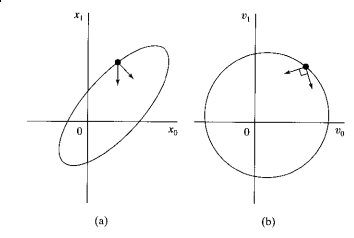
\includegraphics[width=0.5\textwidth]{conjugateVectors.png}
\caption{sujungtiniai vektoriai.}
\label{conjugateVectors}
\end{center}
\end{figure}

Panagrinėkime pavyzdį pateiktą \ref{conjugateVectors} pav.
A dalyje pateikta elipsė atitinkanti dvimatį (\ref{targetFunction}) variantą.
Taip pat pavaizduoti du sujungtiniai vektoriai.
Jeigu matricą $A$ transformuosime taip, kad elipsė taptų apskritimu - sujungtiniai veiktoriai taps statmeni.

\subsection{F(x) optimizavimas}
\label{Foptimizavimas}

Sujungtinių krypčių metodas turimiems $s_{1}, ... , s_{w}$ apibrėžiamas kaip

\begin{equation}
	x_{n + 1} = x_{n} + \eta_{n}s_{n}, \; n = 1, ... , w
\end{equation}

kur $x_{0}$ yra bet koks pradinis vektorius, o $\eta$ yra apibrėžiama kaip

\begin{equation}
	f(x_{n} + \eta_{n} s_{n}) = \min_{\eta} f(x_{n} + \eta s_{n})
\end{equation}

Neformaliai kalbant, sujungtinių krypčių metodas pradeda bet kuriame taške $x_{0}$ ir atlieka $f(x)$ reikšmių "pjūvį" $s_{0}$ kryptimi.
Tuomet tame "pjūvyje" randa mažiausią $f(x)$ reikšmę ir pasirenką tą tašką, kaip naują pradžios tašką.
Toliau tas pats kartojama su likusiais $s$ vektoriais.
Verta pastebėti, kad sujungtinių gradientų metodas reikauja ne daugiau kaip $w$ sujungtinių vektorių minimumo radimui.

\subsection{F(x) iteracinis optimizavimas}
Jau \ref{Foptimizavimas} poskyryje buvo netiesiogiai užsiminta, apie tai, kad šis metodas taikomas iteraciškai.
Sujungtinių vektorių radimui apsibrėšime stačiausio nuolydžio (atvirkštinės išvestinės) krypties funkciją.

\begin{equation}
	r_{n} = b - Ax_{n}
\end{equation}


Vykdant iteracijas, vektorius $s$ apibrėžiamas kaip stačiausio nuolydžio ir prieš tai buvusio sujungtinio vektoriaus tiesinė kombinacija.
\begin{equation}
	s_{n} = r_{n} + \beta_{n} s_{n - 1}
\end{equation}

pradinis sujungtinis vektorius prilyginamas stačiausio nuolydžio krypčiai:
\begin{equation}
	s_{0} = r_{0}
\end{equation}

koeficiento $\beta_{n}$ radimui galima naudoti tiesiogiai išvestą formulę priklausiančią nuo A, tačiau Polak–Ribière, Fletcher–Reeves, Hestenes-Stiefel, Dai–Yuan pasiūlė efektyvesnių variantų.
Čia panagrinėsime Polak–Ribière, Fletcher–Reeves, pasiūlytus variantus.

\paragraph{Polak–Ribière formulė}
Polak–Ribière pasiūlė tokį variantą $\beta_{n}$ radimui:

\begin{equation}
	\beta_{n} = \dfrac {r_{n}^{T} (r_{n} - r_{n-1})} {r_{n-1}^{T} r_{n-1} }
\end{equation}

\paragraph{Fletcher–Reeves formulė}
Fletcher–Reeves pasiūlė tokį variantą $\beta_{n}$ radimui:

\begin{equation}
	\beta_{n} = \dfrac {r_{n}^{T} r_{n} } {r_{n-1}^{T} r_{n-1} }
\end{equation}

Abi šios formulės nenaudoja matricos $A$ dėl ko jų efektyvumas palyginus su įprastais metodais yra geresnis.
Taip pat jos abi yra ekvivaliančios kvadratinei $f(x)$.
Tačiau jeigu jos yra naudojamos atvejams kuomet nuostolių funkcija nėra kvadratinė, bet aproksimuojama (pvz.: atmetant aukštesnio laipsnio dalis) - generuojami $s$ vektoriai nėra tiksliai sujungtiniai ir po keletos iteracijų gali užstrigti.
Dažnai renkamasi Polak–Ribière formulė su apribojimu:

\begin{equation}
	\beta_{n} = max [ \beta_{pr}, 0 ]
\end{equation}

kur $\beta_{pr}$ yra Polak–Ribière $\beta$ iteracijoje $n$.

\subsubsection{Žemiausio taško juostoje radimas}

Turint $s_{n}$ vektorių reikia rasti minimalią $\epsilon(x)$ funkcijos reikšmę jo kryptimi.
Pateikiamas numerinis būdas rasti $\epsilon(x)$ minimalią reikšmę.
Iš pradžių pasirenkame tris taškus taip, kad

\begin{equation}
	\epsilon(\eta_{1}) \geq \epsilon(\eta_{3}) \geq \epsilon(\eta_{2}), \; \text{kur} \: \eta_{1} < \eta_{2} < \eta_{3}
\end{equation}

Tuomet ant šių taškų užbrėžiame kvadratinė kreivę taip, kad ji eitų per visus tris taškus (išsprendžiame kvadratinę lygtį) (žr.: \ref{kvadratineNepatikslinta} pav).

\begin{figure}[H]
\begin{center}
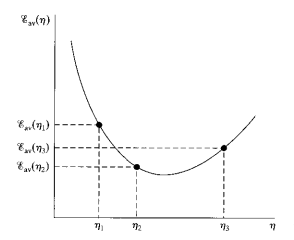
\includegraphics[width=0.5\textwidth]{kvadratineNepatikslinta.png}
\caption{Kvadratine kreivė einanti per tris pasirinktus taškus prieš patikslinimą.}
\label{kvadratineNepatikslinta}
\end{center}
\end{figure}

Tuomet randame šios kvadratinės funkcijos minimumą, ir minimumo tašką priskiriame $\eta_{4}$.
$\eta_{1}$, $\eta_{2}$ ir $\eta_{4}$ naudojame kaip naujus tris taškus minimizavimui.
Toliau kartojame procesą, kol rasta minimumo reikšmė tenkins pasirinktus baigties kriterijus (žr.: \ref{kvadratinePatikslinta} pav).

\begin{figure}[H]
\begin{center}
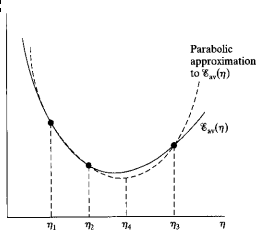
\includegraphics[width=0.5\textwidth]{kvadratinePatikslinta.png}
\caption{Kvadratine kreivė einanti per tris pasirinktus taškus po patikslinimo.}
\label{kvadratinePatikslinta}
\end{center}
\end{figure}

\sectionnonum{Išvados}

Šiame referate buvo aprašytas sujungtinių gradientų metodas dažnai naudojamas įvairiose optimizavimo bei mašinų mokymo uždaviniuose.



\printbibliography[heading=bibintoc]  % Šaltinių sąraše nurodoma panaudota
% literatūra, kitokie šaltiniai. Abėcėlės tvarka išdėstomi darbe panaudotų
% (cituotų, perfrazuotų ar bent paminėtų) mokslo leidinių, kitokių publikacijų
% bibliografiniai aprašai. Šaltinių sąrašas spausdinamas iš naujo puslapio.
% Aprašai pateikiami netransliteruoti.

% \appendix  % Priedai
% Prieduose gali būti pateikiama pagalbinė, ypač darbo autoriaus savarankiškai
% parengta, medžiaga. Savarankiški priedai gali būti pateikiami ir
% kompaktiniame diske. Priedai taip pat numeruojami ir vadinami. Darbo tekstas
% su priedais susiejamas nuorodomis.


\end{document}
